\documentclass[11pt]{article}
\usepackage{icmlko}
\begin{document}

\title{배포가 정한 것 중 하나는 동전이었다 --- 위약이 규약을 통과한다}
\author{월드모델 실험실}
\date{노트 378 · 2026년 8월 1일}
\maketitle

\begin{abstract}
노트 367이 만든 규약은 이렇다: 판 차이가 짝 SD 두 배 안이고 부호가
4/12\,--\,8/12 면 미결정이고, 그때는 \textbf{배포(팝업)가 정한다.} 판이
직접 정할 때는 부호가 9/12 이상이거나 3/12 이하여야 하는데, \textbf{배포가
정할 때는 부호 조건이 없다} --- 차이의 부호만 보면 된다.

노트 377에서 위약 팔을 하나 돌리다 이 구멍이 드러났다. 그 팔은 태거가
비운 칸을 \textbf{중립값 0.5로 채우고 관측 표시자만 켠 것}이라, 하네스가
보는 값 열이 챔피언과 \emph{글자 그대로 같고} 표시자 열만 다르다 ---
정보를 더한 게 아니라 ``이 칸이 비었다''는 사실을 지운 것이다. 그런데
판 $-0.0001$ · 5/12 로 미결정이 되고 팝업이 $+0.0165$ · 7/12 라
\textbf{규약대로면 채택된다.}

그래서 기록에 남은 관문을 다 감사했다. \textbf{배포가 정한 것이 여덟이고,
부호 조건을 넣으면 셋이 바뀐다.} 그중 하나는 이미 챔피언에 들어가 있는
결정이다 --- \texttt{제도메인 재현}(노트 369)이 팝업 $+0.0031$ · 8/12 로
채택됐다.

\textbf{그것을 36뽑기로 다시 쟀다.} 12뽑기에서 8/12(67\%)였던 부호가 18에서
11/18, 24에서 15/24, 30에서 17/30, \textbf{36에서 17/36(47\%)} 이 되고
차이도 $+0.0015 \to -0.0011$ 로 부호가 뒤집힌다. 동전이라는 가설의 이항검정
$p=0.868$ 이다. \textbf{채택의 근거였던 8/12 는 동전이 앞면으로 떨어진
것이었다.}

규약을 고친다: 판이 미결정이면 배포를 보되 \textbf{배포도 9/12 이상 ·
3/12 이하라야 정한다.} 그 사이면 36뽑기로 다시 재고, 36에서도
27/36\,--\,9/36 사이면 \textbf{유지한다}(챔피언이 이긴다).
\end{abstract}

\section{구멍이 어떻게 보였나}

노트 377이 팝업 주장 행을 못 쓰는 이유를 축의 빈 칸으로 좁힌 뒤, 그
빈 칸을 채우는 것이 왜 해로운지 가르려고 팔 셋을 돌렸다 --- 태거 값을
그대로 넣기, 태거의 재현 $\rho$ 만큼 중립 쪽으로 줄여 넣기, 그리고
\textbf{위약}: 중립값 0.5를 넣고 표시자만 켜기.

위약이 정말 정보가 없는지는 하네스가 보는 열로 확인했다.
\texttt{DirectPool.\_feat} 은 축마다 값 열과 표시자 열을 낸다:

\begin{center}
\begin{tabular}{lcccc}
\hline
 & 값 & 표시자 & 값 & 표시자 \\
\hline
챔피언 & 0.3 & 1 & \textbf{0.5} & \textbf{0} \\
위약   & 0.3 & 1 & \textbf{0.5} & \textbf{1} \\
\hline
\end{tabular}
\end{center}

값 열은 완전히 같다 --- 안 채워진 칸은 원래 0.5로 대입되기 때문이다.
\textbf{위약이 바꾸는 것은 표시자뿐이고, 그 표시자를 켜는 것은 ``아무도
이 팝업을 안 태깅했다''는 정보를 지우는 일이다}(노트 124가 그 표지를
만들었다). 정보를 더하지 않고 빼는 팔이다.

\begin{figure}[t]
\centering
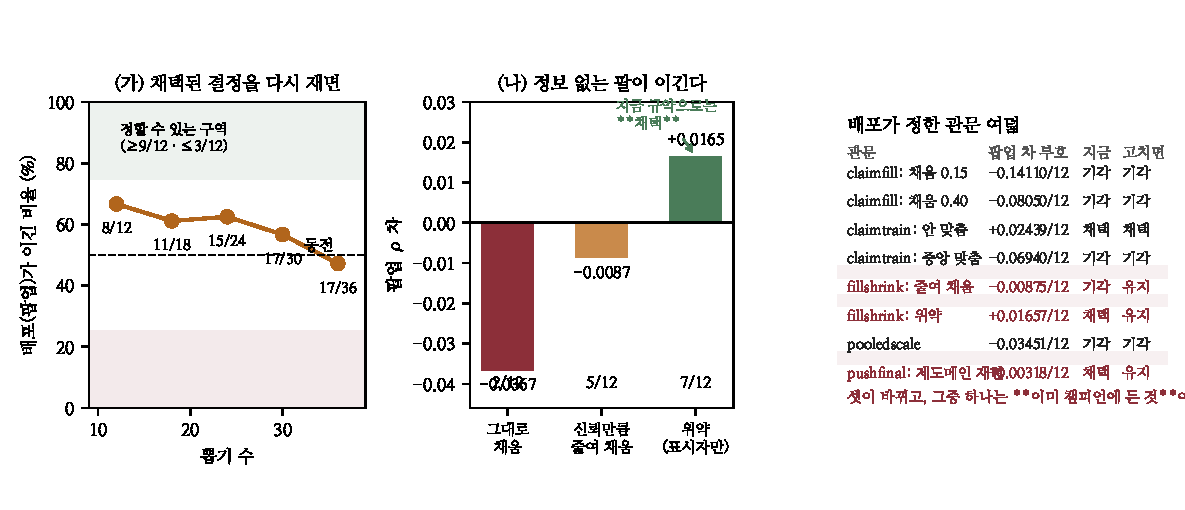
\includegraphics[width=\linewidth]{figs/fig378.pdf}
\caption{\textbf{(가)} 이미 채택된 \texttt{제도메인 재현} 을 뽑기 수를
늘려 다시 쟀다. 채택 근거였던 8/12 가 36뽑기에서 17/36 으로 내려앉고
차이의 부호가 뒤집힌다. \textbf{(나)} 노트 377의 팔 셋. 정보를 빼기만 한
위약이 팝업에서 제일 높고, 지금 규약으로는 채택된다. \textbf{(다)} 기록에
남은 관문 여덟 중 배포가 정한 것 전부. 부호 조건을 넣으면 붉은 셋이
바뀌고, 마지막 줄은 이미 챔피언에 든 결정이다.}
\label{fig:main}
\end{figure}

\section{감사 --- 배포가 정한 여덟}

\begin{center}
\begin{tabular}{lrrll}
\hline
관문 & 팝업 차 & 부호 & 지금 & 부호 조건을 넣으면 \\
\hline
claimfill: 채움 0.15 & $-0.1411$ & 0/12 & 기각 & 기각 \\
claimfill: 채움 0.40 & $-0.0805$ & 0/12 & 기각 & 기각 \\
claimtrain: 안 맞춤 & $+0.0243$ & 9/12 & 채택 & 채택 \\
claimtrain: 중앙 맞춤 & $-0.0694$ & 0/12 & 기각 & 기각 \\
fillshrink: 줄여 채움 & $-0.0087$ & 5/12 & 기각 & \textbf{유지} \\
fillshrink: 위약 & $+0.0165$ & 7/12 & \textbf{채택} & \textbf{유지} \\
pooledscale & $-0.0345$ & 1/12 & 기각 & 기각 \\
pushfinal: 제도메인 재현 & $+0.0031$ & 8/12 & \textbf{채택} & \textbf{유지} \\
\hline
\end{tabular}
\end{center}

셋이 바뀐다. 앞의 둘은 결과가 같다(챔피언 유지). \textbf{마지막 줄만
다르다} --- 그것은 채택돼서 지금 챔피언 안에 있다.

\section{그 하나를 36뽑기로 다시 쟀다}

\texttt{제도메인 재현} 은 노트 369가 공유 열의 눈금을 도메인마다 따로
매기기로 한 결정이다. 그때 판은 $-0.0011$ · 5/12 로 미결정이었고 팝업이
$+0.0031$ · 8/12 라 채택됐다. 같은 두 자료를 그대로 쓰고 뽑기만 늘렸다.

\begin{center}
\begin{tabular}{lrrrr}
\hline
뽑기 & 판 차 & 판 부호 & 팝업 차 & 팝업 부호 \\
\hline
12 & $-0.0008$ & 6/12 & $+0.0015$ & 8/12 (67\%) \\
18 & $-0.0004$ & 8/18 & $+0.0008$ & 11/18 (61\%) \\
24 & $-0.0005$ & 10/24 & $+0.0026$ & 15/24 (63\%) \\
30 & $-0.0001$ & 15/30 & $+0.0010$ & 17/30 (57\%) \\
36 & $-0.0000$ & 20/36 & $\mathbf{-0.0011}$ & \textbf{17/36 (47\%)} \\
\hline
\end{tabular}
\end{center}

부호가 단조로 50\%를 향해 내려오고 36에서 차이의 부호까지 뒤집힌다.
동전이라는 가설의 이항검정이 $p=0.868$ 이다 --- \textbf{구별할 수 없다.}

\textbf{그러면 되돌리나.} 안 되돌린다. 36뽑기가 말하는 것은 ``A가 낫다''가
아니라 ``둘을 구별할 수 없다''이고, 증거가 없기는 되돌리는 쪽도 마찬가지다.
노트 369에는 관문 말고 다른 근거도 있었다 --- 공유 열의 도메인 정체는
원핫이 이미 나르므로 눈금을 합칠 이유가 없고, 원래 유산이 제도메인이었다.
\textbf{다만 이 결정이 관문으로는 동전이었다는 것을 대장에 적는다.}

\section{고친 규약}

\begin{enumerate}
\item 판 차이가 $2\times$짝SD 밖이거나 부호가 9/12 이상 · 3/12 이하면
\textbf{판이 정한다}(방향은 부호가 준다).
\item 아니면 배포(팝업)를 본다. \textbf{배포 부호도 9/12 이상 · 3/12
이하라야 정한다.}
\item 그 사이면 \textbf{36뽑기로 다시 잰다.} 27/36 이상 · 9/36 이하면
정하고, 아니면 \textbf{유지}한다 --- 챔피언이 동점에서 이긴다.
\item 두 팔의 \textbf{채점 집합이 다르면} 미결정이 아니라 \textbf{잴 수
없음}이다(노트 377).
\end{enumerate}

3번이 새 조항이고, 오늘 그것이 실제로 작동하는 것을 봤다 --- 8/12 는
36뽑기에서 17/36 이 됐다.

\textbf{왜 12가 모자란가.} 팝업 유보는 65행이고 짝 SD가 $0.0125$ 인데
재려는 차이가 $+0.0031$ 이다. 차이가 SD의 4분의 1이면 12뽑기의 부호는
평균 7\,--\,8이 나오고 그것은 동전과 구별이 안 된다. \textbf{규약이 부호를
쓰기로 했으면 부호가 감당할 수 있는 크기인지도 물어야 했다.}

\section{남은 것}

\begin{center}
\begin{tabular}{lll}
\hline
항목 & 왜 값이 큰가 & 어떻게 \\
\hline
채택 이력 전수 감사 & 대장 47건 중 관문 기록은 여덟뿐 & 옛 노트의 채택 근거를 훑는다 \\
배포 도메인 자체 & 65행이 판 전체를 정한다 & 팝업 실측 41행 수집 \\
36뽑기 상시화 & 12는 부호를 못 감당한다 & 비용 재고 기본값 올릴지 \\
\hline
\end{tabular}
\end{center}

\end{document}
